\documentclass{article}
\usepackage{tikz}
\usetikzlibrary{decorations.markings}
\pagestyle{empty}
\begin{document}
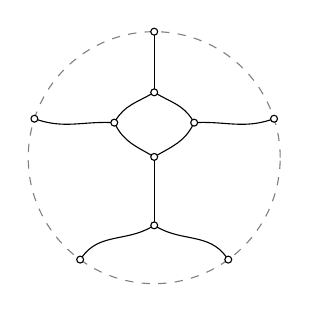
\begin{tikzpicture}
[scale=1.6,every node/.style={draw, circle, fill=white, inner sep=0pt, outer sep=0pt, minimum size=2.5pt},
->-/.style={decoration={markings, mark=at position .5 with{\arrow{>}}}, postaction={decorate}},
-<-/.style={decoration={markings, mark=at position .5 with{\arrow{<}}}, postaction={decorate}}]
\draw[gray, dashed] (0,0) circle (1.0);
 \node (6) at (0.0,1.0) {};
\node (7) at (-0.951057,0.309017) {};
\node (8) at (-0.587785,-0.809017) {};
\node (9) at (0.587785,-0.809017) {};
\node (10) at (0.951057,0.309017) {};
\node (1) at (0.0,0.0062) {};
\node (2) at (-0.317,0.278) {};
\node (3) at (0.0,0.5186) {};
\node (4) at (0.317,0.278) {};
\node (5) at (-0.0,-0.5373) {};
\draw[out=-162.000008, in=2.0] (10) to (4);
\draw[out=125.999988, in=330.0] (9) to (5);
\draw[out=54.000012, in=570.0] (8) to (5);
\draw[out=-17.999992, in=178.0] (7) to (2);
\draw[out=-90.0, in=90.0] (6) to (3);
\draw[out=270.0, in=450.0] (1) to (5);
\draw[out=510.0, in=298.0] (1) to (2);
\draw[out=418.0, in=210.0] (2) to (3);
\draw[out=390.0, in=242.0] (1) to (4);
\draw[out=330.0, in=122.0] (3) to (4);
\end{tikzpicture}
\end{document}